% !TEX root = ./Vorlesungsmitschrift DIFF 2.tex  
\lecture{Do 30.04. 10:15}{}
\section{Äquivalenz von Metriken}
Wir haben gesehen, dass die Eigenschaften derselben Menge sehr verschieden sein können, je nachdem mit welcher Topologie man sie versieht.
\begin{beispiel*}
    \( \reals \) mit der Standardtopologie \( \abs{x-y} \):
    \begin{itemize}
        \item \( \linterval{a}{b} \) ist nicht offen, \( \interval{a}{b} \) ist kompakt.
    \end{itemize}
    \( \reals \) mit der diskreten Metrik \( d_{\text{disk}} \)
    \begin{itemize}
        \item Alle Teilmengen sind offen.
        \item Nur endliche Teilmengen sind kompakt.
        \item Konvergiert \( x_n\goesto a \) (bezüglich \( d_{\text{disk}} \)),so muss gelten \( \exists N \) \sd \( x_n=a\quad \forall n\geq N \) (denn \( \Set{a} \) ist Umgebung von \( a \), oder anders gesagt: damit \( \distance{x_n}{a}<\varepsilon<1 \) wird, muss gelten \( x_n=a \)).
        \item \emph{Alle} Abbildungen \( f\maps (X,d_{\text{disc}})\to (Y,d) \) sind stetig. (Beweis am einfachsten über Folgenstetigkeit).
    \end{itemize}
    Andererseits gilt:\\
    \( U\subset \reals^2 \) ist offen in \( (\reals^2,d_{\text{Eukl}}) \) \tiff \( U \) ist offen in \( (\reals^2, d_{\max}) \).
    \begin{proof}
        \begin{proofdescription}
            \item[\hin] Sei \( a\in U \) \( \overset{VOR}{\implies} \) \texists \( \varepsilon>0 \) \sd
            \begin{align*}
                \ball;{\varepsilon}^{d_\text{E}}(a)\definedas \Set{x\in \reals^2|d_{\text{Eukl}(x,a)}=\sqrt{(x_1-a_1)^2+(x_2-a_2)^2}<\varepsilon}\subset U
            \end{align*} 
        \end{proofdescription}
        Da \( \ball;{\rho}^{d_{\max}}(a)\subset \ball;{\varepsilon}^{d_{\text{E}}}(a) \) für \( \rho=\frac{\varepsilon}{\sqrt{2}} \), ist \( U \) auch offen \( (\reals^2, d_{\max}) \).
        \begin{figure}[H]
            \centering
            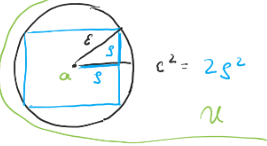
\includegraphics[width=0.5\linewidth]{figures/max_quadrat_in_eukl_kreis}
            \label{fig:max_quadrat_in_eukl_kreis}
        \end{figure}
        \item[\rueck] Sei \( a\in U \)\( \overset{VOR}{\implies} \)\texists \( \varepsilon>0 \) \sd
        \begin{align*}
            \ball;{\varepsilon}^{d_{\max}}(a)=\Set{x|d_{\max}(x,a)<\varepsilon}\subset U.
        \end{align*}
        Es gilt \( \ball;{\rho}^{d_{\text{E}}}(a)\subset \ball;{\varepsilon}^{d_{\max}}(a) \) für \( \rho=\varepsilon \), also ist \( U \) offen in \( (\reals^2,d_{\text{Eukl}}) \).
        \begin{figure}[H]
            \centering
            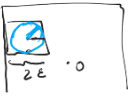
\includegraphics[width=0.4\linewidth]{figures/eukl_kreis_in_max_quadrat}
            \label{fig:eukl_kreis_in_max_quadrat}
        \end{figure}
        
    \end{proof}
    
\end{beispiel*}
\begin{definition}\index{Stärke von Metriken}
    Sei \( X \) eine Menge, seien \( d \) und \( \tilde{d} \) Metriken auf \( X \). Dann nennt man \( d \) \emph{stärker} (feiner) als \( \tilde{d} \), falls jede bezüglich \( \tilde{d} \) offene Menge auch offen bezüglich \( d \) ist, und \emph{schwächer} (gröber), falls \( \tilde{d} \) stärker ist als \( d \). Ist \( d \) sowohl stärker als auch schwächer als \( \tilde{d} \), so nennt man \( d \) und \( \tilde{d} \) \emph{äquivalent}.
\end{definition}
\begin{beispiel*}
    \( d_{\max} \) ist äquivalent zu \( d_{\text{Eukl}} \). \( d_{\text{disk}} \) ist stärker als \( d_{\max}  \) und nicht schwächer.
\end{beispiel*}
\begin{bemerkungen}
    Sei \( d \) stärker als \( \tilde{d} \). Dann gilt:
    \begin{enumerate}
        \item Konvergiert eine Folge bezüglich der stärkeren Metrik, so auch bezüglich der schwächeren.
        
        (denn: Konvergiere \( x_n\to a \) (bezüglich \( d \)). Sei \( \varepsilon>0 \). Betrachte \( \ball;{\varepsilon}^{\tilde{d}}(a)=U \) offen bezüglich \( d \) \timplies \( U \) Umgebung von \( a \) (bezüglich \( d \)) \timplies \( U \) Umgebung von \( a \) (bezüglich \( d \)) \timplies \texists  \( N \) \sd \( x_n\in U\quad \forall n\geq N \).)
        
        \item Ist eine Funktion \( f\maps (X,\tilde{d})\to (Y,d_Y) \) stetig, so auch \( f\maps (X,d)\to (Y,d_Y) \).
        \item Ist eine Funktion \( f\maps (Y,d_Y)\to (X,d) \) stetig, so auch \( f\maps (Y,d_Y)\to (X,\tilde{d}) \).
        
        \begin{proof}
            \( f \) stetig \tiff Urbilder offener Mengen sind offen.
            \begin{proofenumerate}
                \stepcounter{enumi}
                \item \( U\subset Y \) \timplies \( \inverse{f}(U) \) offen bezüglich \( \tilde{d} \) \timplies \( \inverse{f}(U) \) offen bezüglich \( d \).
                \item Sei \( U\subset X \) offen bezüglich \( \tilde{d} \), also auch offen bezüglich \( d \) \timplies \( \inverse{f}(U) \) offen in \( Y \).
            \end{proofenumerate}
            
        \end{proof}
        
    \end{enumerate}
\end{bemerkungen}
\begin{bemerkung*}
    Sind \( d \) und \( \tilde{d} \) äquivalent, sind die selben Folgen konvergent, die selben Mengen offen, kompakt, die selben Funktionen stetig etc.
\end{bemerkung*}
\chapter{Normierte Vektorräume}
\begin{definition}\label{norm}\index{Norm}
    Sei \( V \) ein reeller Vektorraum. Eine \emph{Norm} auf \( V \) ist eine Abbildung \( \norm{\cdot}\maps V\to \reals \) mit
    \begin{eigenschaftenenumerate}
        \item\label{norm:positiv_definit}
        \begin{align*}
            \norm{x}=0\iff x=0
        \end{align*}
        \item \label{norm:betrags_homogen}
        \begin{align*}
            \norm{\lambda x}=\abs{\lambda}\norm{x}\quad \forall \lambda\in \rho,\logicspace x\in V
        \end{align*}
        
        \item \label{norm:dreiecksungleichung}\begin{align*}
            \norm{x+y}\leq \norm{x}+\norm{y}\quad \forall x,y\in V
        \end{align*}
        Dreiecksungleichung.
    \end{eigenschaftenenumerate}
    Ein \emph{normierter VR} \( (V,\norm{\cdot}) \) ist ein VR mit einer Norm.
\end{definition}
\begin{beispiele*}
    \begin{itemize}
        \item \( \reals^n \) mit \( \euclidiannorm{\cdot} \) Euklidische Norm auf \( \reals^n \)
        \begin{align*}
            \norm{x}=\sqrt{\sum_{i=1}^{n}x_i^2}\quad x=(x_{1},\dotsc,x_n).
        \end{align*}
        \item \( \reals^n \) mit \( \supnorm{\cdot}=\explicitnorm{\max}{\cdot} \),
        \begin{align*}
            \supnorm{x}=\Max{\Set{\abs{x_1},\dotsc,\abs{x_n}}}.
        \end{align*}
        \item \( \reals^n \) mit \( \norm{\cdot}_p \) \enquote{\( p \)-Norm}, \( p\geq 1 \), \( p\in \reals \).
        \begin{align*}
            \norm{x}_{p}=\p*{ \sum_{i=1}^{n}\abs{x_i}^p }^{1/p}\quad \to\logicspace  \text{Saalübung}.
        \end{align*}
        \item \( \stetigefunktionen(\interval{a}{b}) \) mit \( \norm{f}_{L^1}=\Integrate{\abs{f(t)}}{t,a,b} \). 
        \item \( \stetigefunktionen(\interval{a}{b}) \) mit \( \supnorm{f}=\sup_{t\in \interval{a}{b}}\abs{f(t)} \). 
    \end{itemize}
\end{beispiele*}
\begin{lemma}
    Sei \( (V,\norm{\cdot}) \) normierter VR\@. Dann wird durch \( \distance{x}{y}\definedas \norm{x-y} \) eine Metrik auf \( V \) definiert (\enquote{induziert}).
\end{lemma}
\begin{proof}
    \ref{norm:positiv_definit} (Norm) \timplies \ref{metrik:nicht_ausgeartet} (Metrik). \ref{metrik:symmetrisch} (Symmetrie der Metrik): folgt aus \( \norm{x-y}=\norm{y-x} \).
\end{proof}
\begin{notation*}
    Wir schreiben \( (V,\norm{\cdot}) \) für den \emph{metrischen} Raum, dessen Metrik von \( \norm{\cdot} \) induziert wird.
\end{notation*}
\begin{bemerkung*}
    Nicht jede Metrik auf einem Vektorraum wird von einer Norm induziert, denn induzierte Metriken erfüllen \( \distance{\lambda x}{\lambda y}=\abs{\lambda}\distance{x}{y} \). Die diskrete Metrik erfüllt das nicht.
\end{bemerkung*}
\begin{lemma}\label{normen_staerke_abschaetzung}
    Seien \( d_1 \) und \( d_2 \) auf \( V \) von Normen \( \norm{\cdot}_1 \) und \( \norm{\cdot}_2 \) induziert. Dann ist \( d_2 \) stärker als \( d_1 \) genau dann, wenn es eine positive Zahl \( C>0 \) gibt \sd
    \begin{align*}
        \norm{x}_1\leq C\norm{x}_2\quad \forall x\in V.
    \end{align*}
\end{lemma}
\begin{proof}
    Bezeichne \( \ball;{r}^j(0) \), \( r>0 \), die offenen Kugeln bezüglich \( d_j \).
    \begin{description}
        \item[\hin] Nach VOR ist insbesondere \( B_1^1(0) \) offen bezüglich \( d_2 \) \timplies \texists \( \varepsilon>0 \) \sd \( B_\varepsilon^2(0)\subset B_1^1(0) \) \timplies für \( x\in X \), \( x\neq 0 \) gilt
        \begin{align*}
            &\norm{\frac{\varepsilon x}{2\norm{x}}_2}_2=\frac{\varepsilon}{2}<\varepsilon\\\
            \implies &\norm{\frac{\varepsilon x}{2\norm{x}_2}}_1 <1 \\
            \implies &\norm{x}_1<\frac{2}{\varepsilon}\norm{x}_2.
        \end{align*} 
        \item[\rueck] Existiere \( C \) wie oben. \( B_r^2(x)\subset \ball;{cr}^1(x)\quad \forall x\in X \), \( r>0 \). Denn \( r>\norm{x-y}_2\geq \frac{1}{c} \). Sei \( U \) offen bezüglich \( d_1 \)
        \begin{align*}
            \implies &\forall x\in U\logicspace \exists \varepsilon>0\logicspace\text{\sd} \logicspace \ball;{\varepsilon}^1(x)\subset U\\
            \implies &\ball;{\frac{\varepsilon}{C}}^2(x)\subset \ball;{\varepsilon}^1(x)\subset U.
        \end{align*} 
    \end{description}
    
\end{proof}
\begin{folgerung*}
    \( d_2 \) ist äquivalent zu \( d_1 \)
    \begin{align*}
        \iff \exists C,\tilde{C} \logicspace\text{\sd} \tilde{C}\norm{x_2}\leq \norm{x_1}\leq C\norm{x_2},
    \end{align*}
    (\enquote{die Normen sind äquivalent}).
\end{folgerung*}
\begin{bemerkung*}
    Äquivalenz von Normen ist eine Äquivalenz-Relation (reflexiv, symmetrisch, transitiv).
\end{bemerkung*}
\begin{bemerkung*}
    Für allgemeine Metriken kann man nicht so eine einfache Abschätzung angeben. Etwa ist \( \reals^n\times \reals^n\ni (x,y)\mapsto \norm{x-y}_{\max} \) unbeschränkt, aber \( d_{\text{discrete}}(x,y)=1\quad \forall x\neq y \). Die Beweisrichtung \rueck gilt noch (also gibt es ein \( C \) wie in \ref{normen_staerke_abschaetzung}, so ist \( d_2 \) stärker als \( d_1 \)). Die Beweisrichtung \hin verwendet die Skalar-Multiplikation des zugrunde liegenden Vektorraums und vor allem die \enquote{Betrags-Homogenität} der Norm
    \begin{align*}
        \norm{\frac{x}{\norm{x}_2}}=\frac{1}{\norm{x}_2}\norm{x}_1.
    \end{align*}
\end{bemerkung*}
\begin{satz}\label{r_alle_normen_aequivalent}
    Auf \( \reals^n \) sind alle Normen äquivalent.
\end{satz}
\begin{proof}
    Aufgrund der Transitivität genügt es die Äquivalenz einer beliebigen Norm \( \norm{\cdot} \) zu \( \supnorm{\cdot} \) zu beweisen.
    \begin{proofenumerate}
        \item \( \supnorm{\cdot} \) ist stärker als \( \norm{\cdot} \):
        Denn sei \( x=\sum_{j=1}^{n}x_j e_j\in \reals^n  \), \( e_j=(0,\dotsc, \underset{j \text{-te}}{1},\dotsc,0) \). Dann ist
        \begin{align*}
            \norm{x}=\norm{\sum x_j e_j}\explain{\triangle \text{und Homog.}}{\leq}\abs{x_j}\cdot\norm{e_j}\leq \supnorm{x}\underbrace{\sum_{j=1}^{n}\norm{e_j}}_{=C}
        \end{align*}
        \item \( \supnorm{\cdot} \) ist schwächer als \( \norm{\cdot} \):
        
        Betrachte \( M\definedas \Set{x\in \reals^n|\supnorm{x}=1} \) (Einheits\enquote{sphäre} bezüglich \( \supnorm{\cdot} \), also Rand des Einheitswürfels 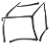
\includegraphics[height=\baselineskip]{figures/einheitswuerfel_rand}).

        \begin{behauptung*}
            \( f\maps M\to \reals \), \( x\mapsto \norm{x} \) ist stetig bezüglich \( \supnorm{\cdot} \).
        \end{behauptung*}
        \begin{subproof}
            \begin{align*}
                \abs{f(x)-f(y)}=\abs{\norm{x}-\norm{y}}\underset{(*)}{\leq}\norm{x-y}\leq C\supnorm{x-y}
            \end{align*}
            \( (*) \) umgekehrte Dreiecksungleichung:
            \begin{align*}
                \norm{x}-\norm{y}&=\norm{x+y-y}-\norm{y}\overset{\triangle}{\leq}\norm{x+y}\\
                \norm{y}-\norm{x}&=\norm{y+x-x}-\norm{x}\leq \norm{x+y}.
            \end{align*}
        \( M \) ist abgeschlossen bezüglich \( \supnorm{\cdot} \) (denn \( \reals^n\setminus M= \) Urbild der offenen Menge \( \reals\setminus \Set{1} \) unter der stetigen Abbildung \( x\mapsto \supnorm{\cdot} \)). \( M\subset  \) abgeschlossenen \emph{Quader} und dieser ist \emph{kompakt} in \( (\reals^n,\supnorm{\cdot}) \) (\thref{quader_ist_kompakt_norm_undendlich}) \timplies \( M \) ist kompakt (\ref{abgeschlossene_teilmenge_kompakter_menge_ist_kompakt}).

        Es folgt: \( f \) nimmt sein Minimum \( b \) an und (da \( f>0 \)) somit ist \( b>0 \). Nach Definition ist \( \norm{y}\geq b\quad \forall y\in M \). Für alle \( x\in \reals^n\setminus\Set{0} \) gilt \( \frac{x}{\supnorm{x}}\in M \), also ist \( \norm{\frac{x}{\supnorm{x}}}\geq b \), also \( \norm{x}\geq b\supnorm{x} \) und für \( x=0 \) gilt dies ohnehin.
        \end{subproof}
    \end{proofenumerate}
\end{proof}
\begin{lemma}\label{quader_ist_kompakt_norm_undendlich}
    Der Quader \( Q=\Set{x=(x_1,\dotsc, x_n)\in \reals^n| a_j\leq x_j\leq b_j} \) ist kompakt in \( \reals^n,\supnorm{\cdot} \) (\( a_j\leq b_j \)).
\end{lemma}
\begin{proof}
    Sei \( (U_j)_j \) eine offene Überdeckung von \( Q \). Angenommen, \( Q \) kann nicht durch endlich viele \( U_j \)'s überdeckt werden.

    Wir konstruieren induktiv eine Folge von abgeschlossenen Teilquadern
    \begin{align*}
        Q_0\supset Q_1\supset Q_2\supset \dotsb
    \end{align*}
    mit
    \begin{eigenschaftenenumerate}
        \item \( Q_n \) kann \emph{nicht} durch endlich viele \( U_j \)'s überdeckt werden
        \item \( \diameter-{Q_m}=2^{-m}\diameter-{Q} \).
    \end{eigenschaftenenumerate}
    \minisec{Beachte:} \( \diameter-{Q}= \) Länge der länsten Seite bezüglich \( \supnorm{\cdot} \).
    \begin{figure}[H]
        \centering
        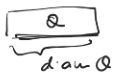
\includegraphics[width=0.3\linewidth]{figures/diameter_quader_norm_unendlich}
        \label{fig:diameter_quader_norm_unendlich}
    \end{figure}
    Setze \( Q_0=Q \). Sei \( Q_m \) konstruiert. Schreibe \( Q_m=I_1\times\dotsb\times I_n \), \( I_j \) abgeschlossene Intervalle. Zerlege \( I_j^{(1)}\cup I_j^{(2)} \) in zwei abgeschlossene Intervalle der halben Länge und setze
    \begin{align*}
        Q^{(s_1,\dotsc,s_n)}\definedas I_1^{(s_1)}\times\dotsb\times I_n^{(s_n)},\quad s_j\in \Set{1,2}.
    \end{align*}
    Das ergibt \( 2^n \) Quader mit
    \begin{align*}
        \bigcup_{s_j\in \Set{1,2}}Q_m^{(s_1,\dotsc,s_n)}=Q_m
    \end{align*}
    \begin{figure}[H]
        \centering
        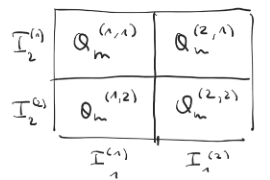
\includegraphics[width=0.5\linewidth]{figures/teilquader}
        \label{fig:teilquader}
    \end{figure}
    Es gibt mindestens einen Quader \( Q_m^{(s_1,\dotsc,s_n)} \), der nicht durch endlich viele \( U_j \)'s überdeckt werden kann. Einen solchen wählen wir als \( Q_{m+1} \). Es gilt per Konstruktion
    \begin{align*}
        \diameter{Q_{m+1}}=\frac{1}{2}\diameter{Q_m}=\frac{1}{2^{m+1}}\diameter{Q}.
    \end{align*}
    
    Nach dem Schachtelungsprinzip \texists \( a\in Q_m \) \tforall \( m \). Da \( (U_j)_j \) \( Q \) überdeckt \texists \( U_{j_0} \) \sd \( a\in U_{j_0} \). \( U_{j_0} \) offen \timplies \texists \( \varepsilon>0 \) \sd \( \ball;{\varepsilon}^{\supnorm{\cdot}}(a)\subset U_{j_0} \). Wähle \( m \) so groß, dass \( \diameter{Q_m}<\varepsilon \). \( a\in Q_m \) \timplies \( Q_m\subset \ball;{\varepsilon}^{\supnorm{\cdot}}(a)\subset U_{j_0} \) \contra Widerspruch Konstruktion der \( Q_m \).
\end{proof}
\begin{bemerkung}
    Aus \ref{r_alle_normen_aequivalent} folgt: \( Q \) ist bezüglich jeder Norm kompakt. Bolzano-Weierstraß (\ref{bolzanoweierstrass}) \timplies In \( (\reals^n,\norm{\cdot}) \) hat jede beschränkte Folge eine konvergente Teilfolge.
\end{bemerkung}
\begin{bemerkungen}
    Wir haben bereits gesehen:
    \begin{enumerate}
        \item Auf nicht endlich-dimensionalen Vektor-Räumen sind nicht alle Normen äquivalent:\\
        \( (\stetigefunktionen(\interval{a}{b}), \supnorm{\cdot}) \) ist vollständig, \( (\stetigefunktionen(\interval{a}{b}), \norm{\cdot}_{L^1}) \) nicht.
        \item Auf dem \( \reals^n \) sind nicht alle Metriken äquivalent: \( d_{\text{disc}} \) ist stärker als jede Norm (und nicht schwächer).
    \end{enumerate}
\end{bemerkungen}
\begin{satz}[Heine-Borel]\label{heineborel}
    Eine Teilmenge \( A\subset \reals^n \) ist genau dann kompakt, wenn sie abgeschlossen und beschränkt ist. (\( \reals^n \) hier und im Folgenden als normierter VR). 
\end{satz}
\begin{proof}
    \begin{proofdescription}
        \item[\hin] Hatten wir letztes Mal (\ref{kompakt:abgeschlossen_beschraenkt}) für Kompakte in metrischen Räumen bewiesen.
        
        \item[\rueck] It \( A \) beschränkt so ist \( A \) in einem Quader enthalten (denn \( \supnorm{x-y}\leq  \norm{x-y} \) somit \( \normdiameter{\supnorm{\cdot}}{A}\leq C\normdiameter{\norm{\cdot}}{A}<\infty \)). \( Q \) ist kompakt (bezüglich \( \supnorm{\cdot} \) somit bezüglich \( \norm{\cdot} \)).\( A \) abgeschlossen \timplies \( A \) kompakt (\ref{abgeschlossene_teilmenge_kompakter_menge_ist_kompakt}).
    \end{proofdescription}
\end{proof}
\begin{bemerkung*}
    \ref{heineborel} gilt nicht in unendlich-dimensionalen Vektorräumen:

    Betrachte in \( \ell_1, \norm{\cdot}_{\ell_1}=\sum_{k=0}^{\infty}\abs{x_k} \) die Folge \( (x^n)_n \) wobei \( x^n=(x^n_k)_k \) sei mit \( x^n_k=0 \) für \( n\neq k \) und \( (x^n)_n=1 \). Dann gilt \( \norm{x^n}_{\ell_1}=1 \) und
    \begin{align*}
        \norm{x^n-x^m}_{\ell_1}=2\quad \forall m\in \Set{0,1,\dotsc,n-1}.
    \end{align*}
    \timplies Die Folge besitzt keine konvergente Teilfolge, kann also (Bolzano-Weierstrass) nicht kompakt sein, obwohl \( \Set{x^n|n\in \naturals_0} \) beschränkt und abgeschlossen in \( (\ell_1, \norm{\cdot}_{\ell_1}) \) ist.
\end{bemerkung*}
